
\usepackage{fancyhdr}
\usepackage{lastpage}
\usepackage[utf8]{inputenc}

% Minted for syntax highliting
\usepackage{minted}
\usemintedstyle{tango}

% 
\usepackage[T1]{fontenc}
\usepackage{lmodern}

\usepackage{calc}
\usepackage{bytefield}

\usepackage{listings}
\usepackage{amsmath}

\usepackage{tikz}
\usetikzlibrary{automata,arrows,topaths,calc,positioning}
 
\usepackage{syntax}
\grammarindent=2cm


% Headers/footers styling
\pagestyle{fancy}
\fancyhf{}
\renewcommand{\headrulewidth}{0pt}

% Footer
\lfoot{ID1019}
\cfoot{KTH}
\rfoot{\thepage \hspace{1pt} / \pageref{LastPage}}

%\newcommand{\defaultpagestyle}{\thispagestyle{plain}}
\newcommand{\defaultpagestyle}{\thispagestyle{fancy}}



\usepackage{pgf-umlsd}
\usepgflibrary{arrows} % for pgf-umlsd
\usetikzlibrary{fit, positioning}

\title[ID1019 A game of Pong]{A game of Pong}


\author{Johan Montelius}
\institute{KTH}
\date{\semester}

\begin{document}

\begin{frame}
\titlepage
\end{frame}

\begin{frame}{the classical game of Pong}

  \begin{figure}
    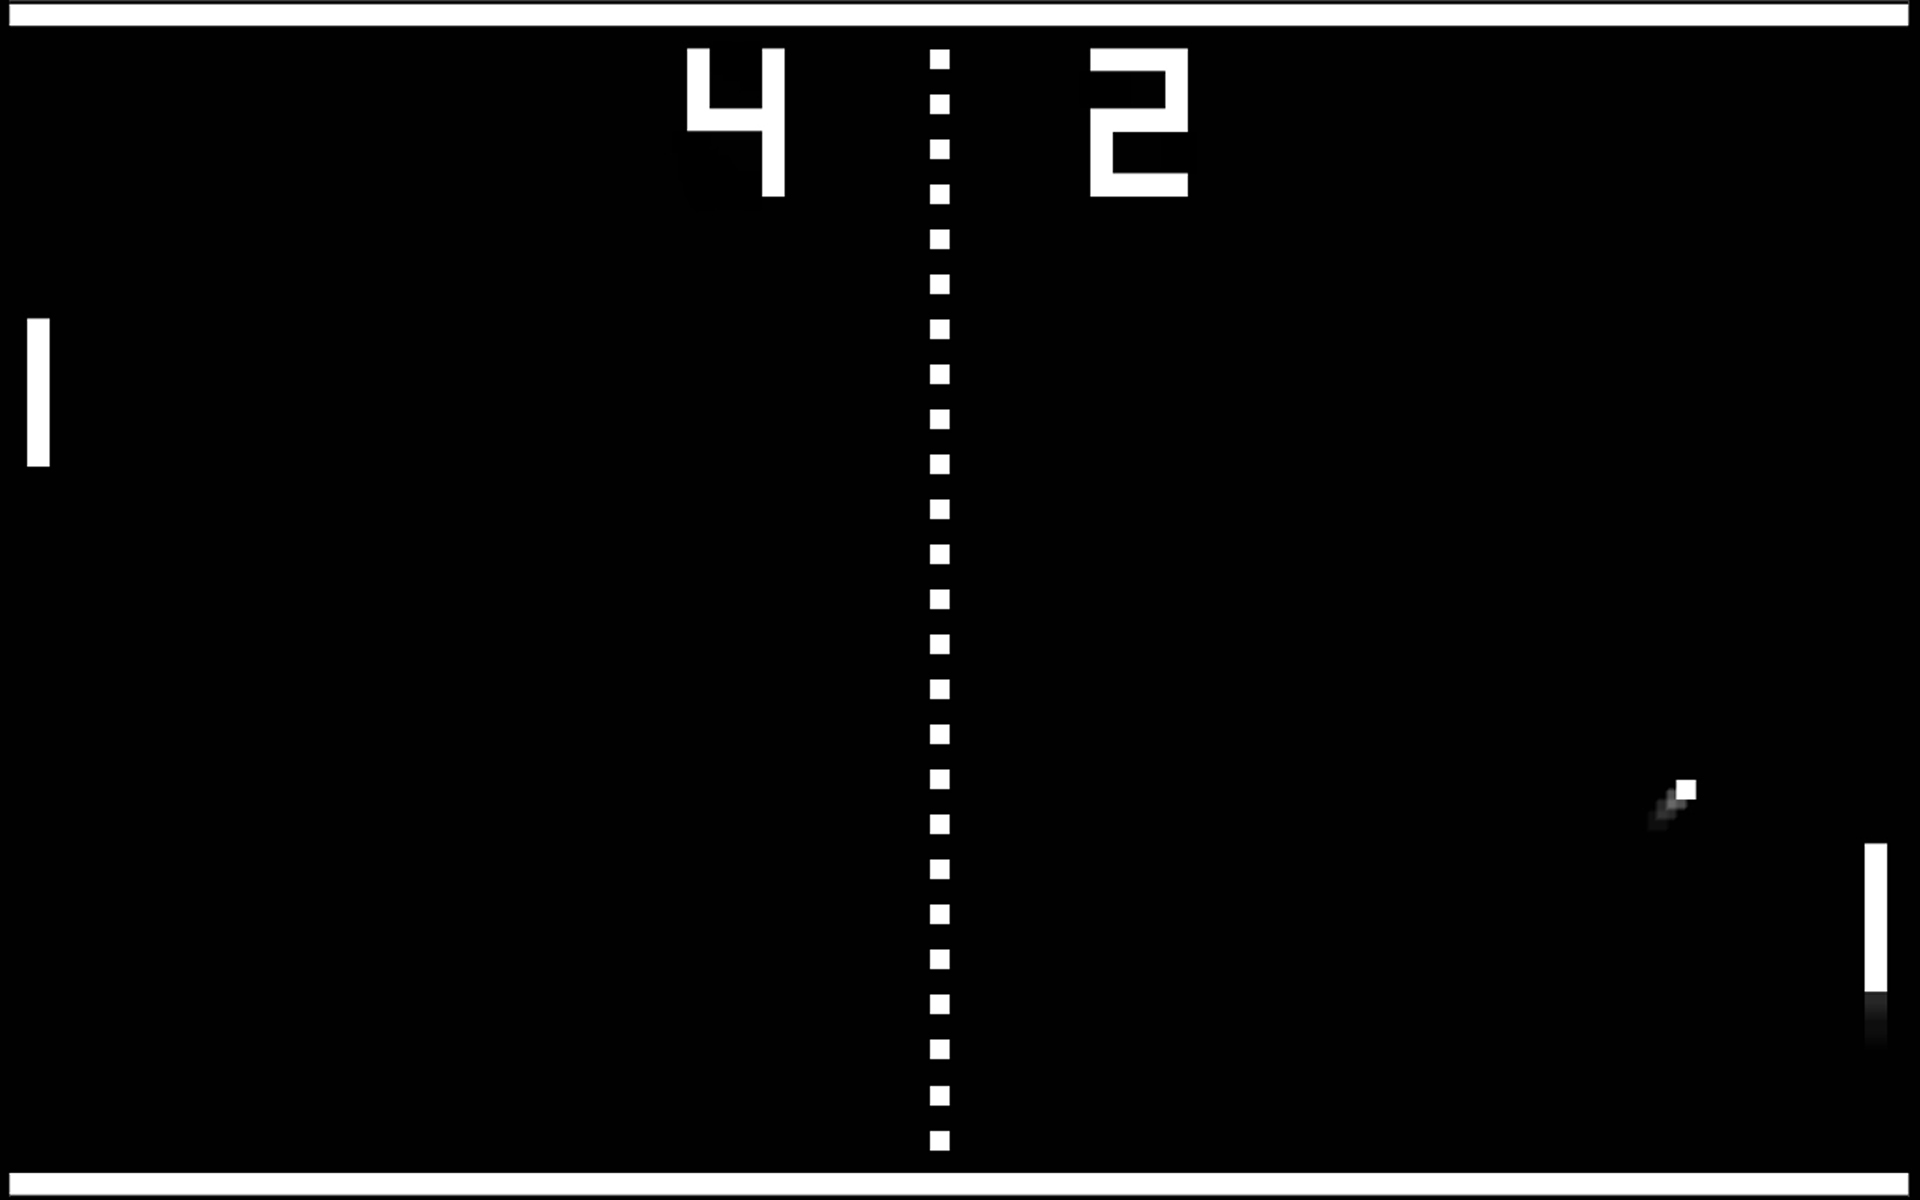
\includegraphics[scale=0.1]{pong.png}
  \end{figure}
  
\end{frame}

\begin{frame}{architectur}

\begin{figure}
  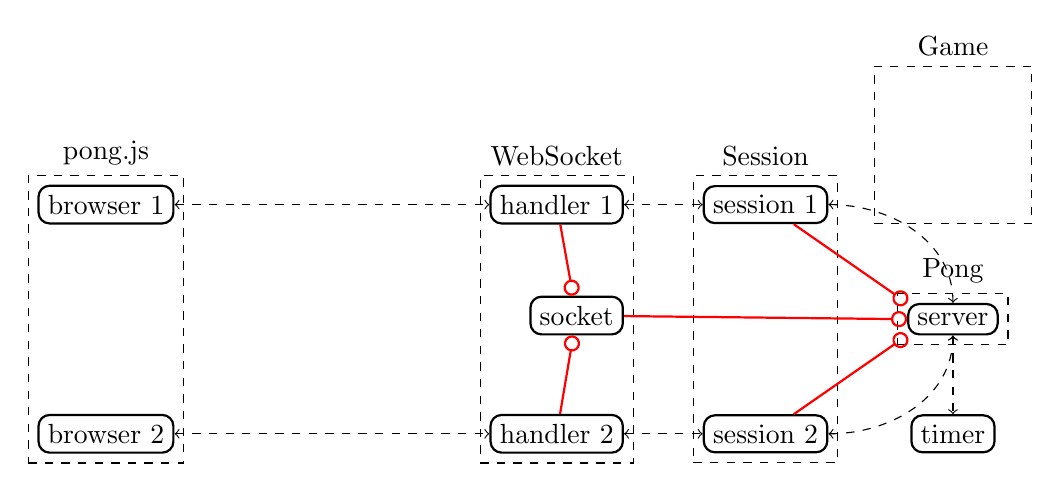
\begin{tikzpicture}
    \node[draw, thick, rounded corners] (server) at (0,0) {server};
    \node[draw, thick, rounded corners, above left = of server] (ses1) {session 1};
    \node[draw, thick, rounded corners, below left = of server] (ses2) {session 2};
    \node[draw, thick, rounded corners, below left = of ses1, above left = of ses2] (socket) {socket};
    \node[draw, thick, rounded corners, left = of ses1] (hdlr1) {handler 1};
    \node[draw, thick, rounded corners, left = of ses2] (hdlr2) {handler 2};
    \node[draw, thick, rounded corners, left = 4.0 cm of hdlr1] (brw1) {browser 1};
    \node[draw, thick, rounded corners, left = 4.0 cm of hdlr2] (brw2) {browser 2};
    \node[draw, thick, rounded corners, below = of server] (tmr) {timer};    

    \node[draw, dashed, fit = (server), label=Pong] {};
    \node[draw, dashed, fit = (ses1)(ses2), label=Session] {};
    \node[draw, dashed, fit = (socket)(hdlr1)(hdlr2), label=WebSocket] {};
    \node[draw, dashed, fit = (brw1)(brw2), label=pong.js] {};

    \node[draw, dashed, rectangle, label=Game, above = of server, minimum size=2cm] {};
    
    \draw[o-,thick, red] (server.west) -- (socket);
    \draw[o-,thick, red] (socket) -- (hdlr1);
    \draw[o-,thick, red] (socket) -- (hdlr2);
    \draw[o-,thick, red] (server.north west) -- (ses1);
    \draw[o-,thick, red] (server.south west) -- (ses2);            

    \draw[<->,dashed, black] (brw1) -- (hdlr1);
    \draw[<->,dashed, black] (brw2) -- (hdlr2);                    

    \draw[<->,dashed, black] (hdlr1) -- (ses1);    
    \draw[<->,dashed, black] (hdlr2) -- (ses2);

    \draw[<->,dashed, black] (ses1.east) to [out=0,in=90] (server.north);
    \draw[<->,dashed, black] (ses2.east) to [out=0,in=270] (server.south);
    \draw[<->,dashed, black] (server.south) to [out=270,in=90] (tmr.north);            


    
  \end{tikzpicture}
\end{figure}

\end{frame}

\begin{frame}{layers of communication}

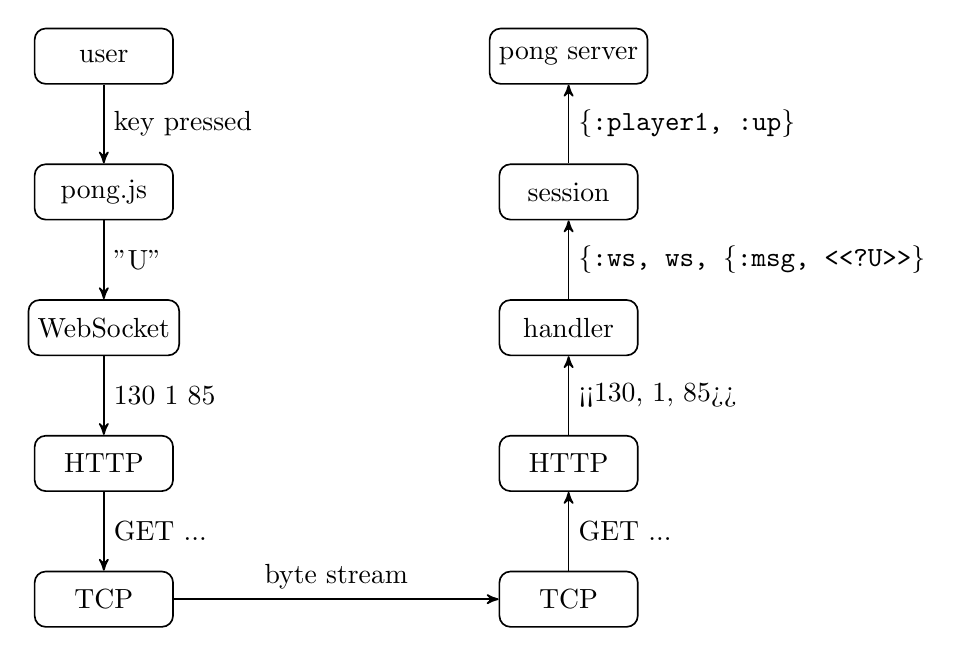
\begin{tikzpicture}[>=stealth', semithick, auto]

    \tikzstyle{fbp} = [rectangle, rounded corners, minimum width=50pt, minimum height=20pt, text centered, draw=black]        


    \node (user)    [fbp]                               {user};
    \node (server)  [fbp, right=4cm of user]            {pong server};            
    
    \node (ses1)    [fbp, below=1cm of user]            {pong.js};
    \node (ses2)    [fbp, below=1cm of server]          {session};        

    \node (ws1)     [fbp, below=1cm of ses1]            {WebSocket};
    \node (ws2)     [fbp, below=1cm of ses2]            {handler};        

    \node (http1)   [fbp, below=1cm of ws1]             {HTTP};
    \node (http2)   [fbp, below=1cm of ws2]             {HTTP};

    \node (tcp1)    [fbp, below=1cm of http1]           {TCP};
    \node (tcp2)    [fbp, below=1cm of http2]           {TCP};    

    \path[->]  (user)    edge        node          {key pressed}                         (ses1);
    \path[<-]  (server)  edge        node          {{\tt \{:player1, :up\}}}             (ses2);
    
    \path[->]  (ses1)    edge        node          { "U" }                               (ws1);
    \path[<-]  (ses2)    edge        node          { {\tt \{:ws, ws, \{:msg, <<?U>>\}}}  (ws2);
    
    \path[->]  (ws1)     edge        node          {130 1 85}                            (http1);
    \path[<-]  (ws2)     edge        node          {<<130, 1, 85>>}                      (http2);

    \path[->]  (http1)   edge        node          {GET ...}                             (tcp1);
    \path[<-]  (http2)   edge        node          {GET ...}                             (tcp2);

    \path[->]  (tcp1)    edge        node          {byte stream}                         (tcp2);

\end{tikzpicture}


\end{frame}


\begin{frame}{sequence diagram}


\begin{figure}
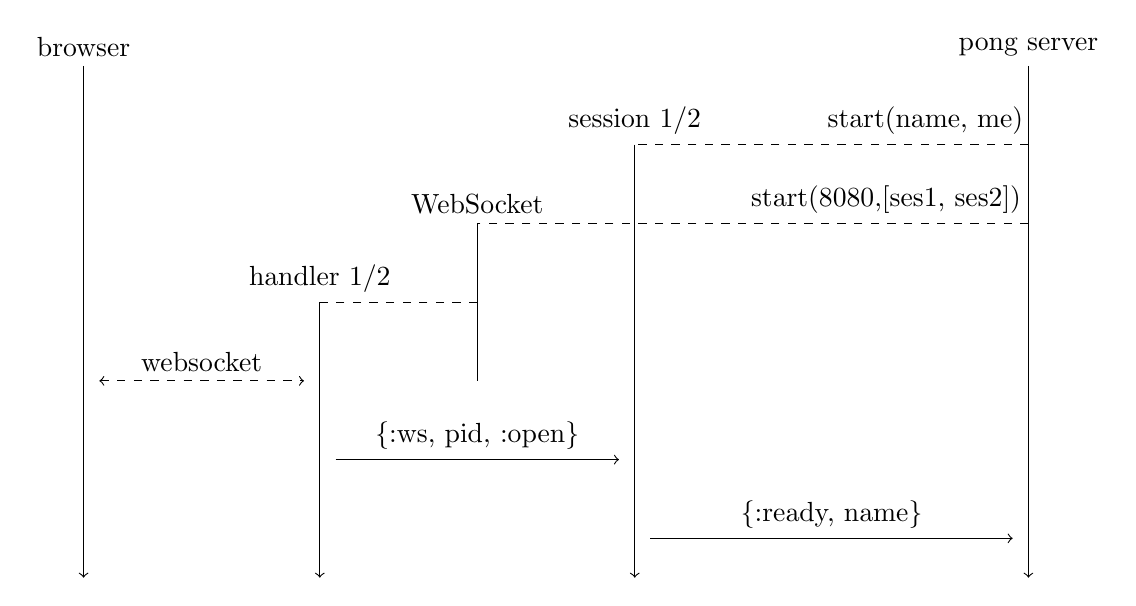
\begin{tikzpicture}

  \coordinate (n0) at (0,6);
  \coordinate (nn) at (0,-0.5);

  \coordinate (a0) at (3, 3);
  \coordinate (an) at (3,-0.5);

  \coordinate (b0) at (5,4);
  \coordinate (bn) at (5,-0.5);

  \coordinate (c0) at (7,5);
  \coordinate (cn) at (7,-0.5);

  \coordinate (s0) at (12,6);
  \coordinate (sn) at (12,-0.5);


  \draw[->] (n0) to []  (nn);
  \draw[->] (s0) to []  (sn);

  \node[anchor=south] at (n0) {browser};
  \node[anchor=south] at (s0) {pong server};

  \pause

  \pause
  \coordinate (s2) at ($(s0)+(0,-1)$);
  \draw[dashed] (s2) -- node[near start, above]{start(name, me)\ \ } (c0);
  \node[anchor=south] at (c0) {session 1/2};  
  \draw[->] (c0) to []  (cn);

  \pause
  
  \coordinate (s3) at ($(s2)+(0,-1)$);
  \draw[dashed] (s3) -- node[near start, above]{start(8080,[ses1, ses2])\ \ } (b0);
  \node[anchor=south] at (b0) {WebSocket};  
  \draw[] (b0) to []  ($(b0)+(0,-2)$);

  \pause

  \coordinate (b1) at ($(b0)+(0,-1)$);
  \draw[dashed] (b1) -- (a0);        
  \node[anchor=south] at (a0) {handler 1/2};  
  \draw[->] (a0) to []  (an);  

  \pause

  \coordinate (n4) at ($(n0)+(0,-4)$);
  \coordinate (a1) at ($(a0)+(0,-1)$);
  \draw[dashed, <->, shorten <=0.2cm, shorten >=0.2cm] (n4) -- node[midway, above] {websocket} (a1);

  \pause
  \coordinate (a2) at ($(a1)+(0,-1)$);
  \coordinate (c2) at ($(c0)+(0,-4)$);
  \draw[->, shorten <=0.2cm, shorten >=0.2cm] (a2) -- node[midway, above] {\{:ws, pid, :open\}} (c2);

  \pause
  \coordinate (c3) at ($(c2)+(0,-1)$);
  \coordinate (s4) at ($(s3)+(0,-4)$);
  \draw[->, shorten <=0.2cm, shorten >=0.2cm] (c3) -- node[midway, above] {\{:ready, name\}} (s4);  


\end{tikzpicture}

\end{figure}
\end{frame}


\begin{frame}{WebSocket interface}

   
  \onslide<1->{The Javascript client communicate using a websocket interface. After
  the initial HTTP handshake, a bidirectional message channel is
  created. Each message consist of sequence of bytes.}

  \vspace{10pt}
  
  
  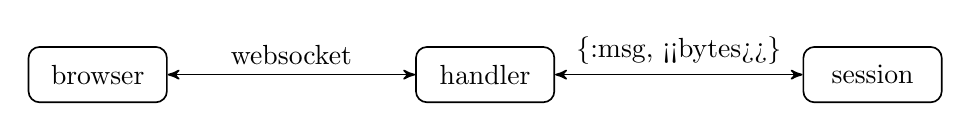
\begin{tikzpicture}[>=stealth', node distance=140pt, semithick, auto]

        \tikzstyle{fbp} = [rectangle, rounded corners, minimum width=50pt, minimum height=20pt,text centered, draw=black]        

        \onslide<2->{
          \node (brw1) [fbp] {browser};
          \node (hdlr1) [fbp, right of=brw1] {handler};

          \path[<->]  (brw1) edge   node      {websocket}       (hdlr1);
        }
        \onslide<3-> {
          \node (ses1) [fbp, right of=hdlr1] {session};
          \path[<->]  (hdlr1) edge   node      {\{:msg, <<bytes>>\}}       (ses1);
        }
\end{tikzpicture}

  \vspace{10pt}

  \onslide<3->{The handler process will take care of the WebSocket
  internals and deliver a stream of messages to the session process.}

  \vspace{10pt}
  
  \onslide<4->{Each client is connected through a unique handler process that is
  communicating with a single session process.}

\end{frame}

\begin{frame}{Session handler lower interface}

Messages from the websocket handler to the session handler:

\vspace{10pt}  \pause

\begin{itemize}
\item {\tt \{:ws, pid, :open\}}  : a connection was establishes
\item {\tt \{:ws, pid, :close\}}  : the connection was closed by the client
\item {\tt \{:ws, pid, \{:msg,  <<byte encoded message>>\}\}} : message from the client
\end{itemize}

\vspace{10pt}  \pause

Messages from the session handler to the websocket handler:

\begin{itemize}
\item {\tt \{:frw, <<byte encoded message>>\}}  : encode and send message to client
\item {\tt :stop} : time to close the connection
\end{itemize}

\end{frame}

\begin{frame}{The session handler}

  Works as a decoder/encoder of byte-encoded  messages and Elixir messages.

  \vspace{20pt}  \pause

  Messages from the client forwarded to the pong game server:

  \vspace{20pt}

  \begin{itemize}
  \item {\tt <<?U>>}  : player pressed up -  {\tt \{name, :up\}}
  \item {\tt <<?D>>}  : player pressed down -  {\tt \{name, :down\}}        
  \end{itemize}


\end{frame}

\begin{frame}{session handler}

  Messages from pong server forwarded to the websocket handler:

  \vspace{20pt}
      
  \begin{itemize}
  \item {\tt \{:player1, :up\}}  : player moved up -  {\tt <<?P,?U>>}
  \item {\tt \{:player1, :down\}}  : player moved down - {\tt <<?P,?D>>}
  \item {\tt \{:player1, :score, score\}}  : player scored - {\tt <<?P,?S, score>>}
  \item {\tt \{:player2, ... \}} : same messages for opponent -  {\tt <<?O, ... >>}        
  \item {\tt \{:ball, x, y \}} : ball moved to new position - {\tt <<?B, x::16, y::16 >>}        
  \item {\tt \{:frw, msg\}}  : raw message to client - {\tt msg}
  \end{itemize}
\end{frame}

\begin{frame}{the game engine}

  The game server:
  \vspace{10pt} \pause
  \begin{itemize}
  \item create two session handlers with unique names \pause
  \item create a WebSocket process, give session handlers as arguments \pause
  \item wait for session handlers to report \pause
  \item start the game \pause
  \end{itemize}
  
\end{frame}


\begin{frame}{the game engine}

  The pong engine keeps a state consisting of:

  \vspace{10pt} \pause
  
  \begin{itemize}
  \item Two players ({\tt player1} and {\tt player2}). \pause
  \item A ball. \pause
  \item The current score.\pause
  \item Two {\em session pids} to send messages to the players. 
  \end{itemize}

  \vspace{10pt} \pause

  The pong engine is defined by two modules: 
  
  \vspace{10pt} \pause
  \begin{itemize}
  \item The Pong module that describes the server as a communicating process. 
  \item The Game module that describe the rules as functions. 
  \end{itemize}
  

\end{frame}


\begin{frame}{Rules of the game}

  \pause A player is represented as a tuple {\tt \{name, x-pos, y-pos, dir\}}.
  \vspace{10pt}

  \begin{itemize}
  \item {\tt player1(name) } : return a named {\tt player 1} 
  \item {\tt player2(name) } : return a named {\tt player 2}  \pause   
  \item {\tt up(player) } : return either {\tt \{:ok, player\}} or {\tt :no} 
  \item {\tt down(player) } : return either {\tt \{:ok, player\}} or {\tt :no} \pause
  \end{itemize}
  \vspace{10pt}      
  \pause A ball is represented a as tuple {\tt \{:ball, x, y, dx, dy\}}.  \pause
  \vspace{10pt}      
  \begin{itemize}
  \item {\tt serve(player)} : return {\tt \{pos, ball\}} \pause
  \item {\tt move_ball(player1, player2, ball)} : return either \pause
    \begin{itemize}
      \item {\tt \{:bounce, pos, ball\}}  (increase speed) \pause
      \item {\tt \{:moved, pos, ball\}} \pause
      \item {\tt \{:score, name\}}\pause
    \end{itemize}
  
  \end{itemize}
  
\end{frame}

\begin{frame}{the Game module}

  The Game module provides only functions; it does not keep a state. 

  \vspace{20pt}\pause
  The Game module knows how large the court is.
  
  \vspace{20pt}\pause
  The state (apart from the score) is held by the three data structures: player1, player2 and the ball.

\end{frame}

\end{document}



